\chapter{全息张量网络中的算符推移}
\label{chap:operator-pushing}

在本章中,我们将沿着第 \ref{chap:strange-correlator} 章的思路,继续考察基于拓扑序的重整化张量网络。这类张量网络可以揭示出对应 CFT 的性质,并且在数值上还可以看到重整化张量与 AdS 体的相似性。因此,研究其中的算符推移及演生广义自由场的条件具有重要意义。

\section{广义自由场与算符推移}

AdS/CFT 对应\cite{maldacena1999large}中的一项重要特征是在 AdS 体 (bulk) 中演生出的\emph{自由场} (free field)。这使得我们可以为体态提供一套半经典的描述,同时也可以通过体来计算边界 CFT 中的物理量。这里所谓“自由场”,是指其关联函数可以通过 Wick 缩并来计算。一般来说,边界 CFT 中的\emph{单迹算符} (single trace operator) 近似对应了半经典的体态理论中的自由 Gauss 场。这就使得 CFT 中的关联函数可以在 AdS 一侧通过 Witten 图来计算\cite{witten1998anti,gubser1998gauge}。也有很多工作探讨了全息 CFT 中所演生出的广义自由场\cite{dutsch2003generalized,liu2019dimensional,collier2019quantum,nebabu2023bulk}。

\begin{figure}[htb]
  \centering
  \subcaptionbox{\label{fig:rt-formula}}{%
    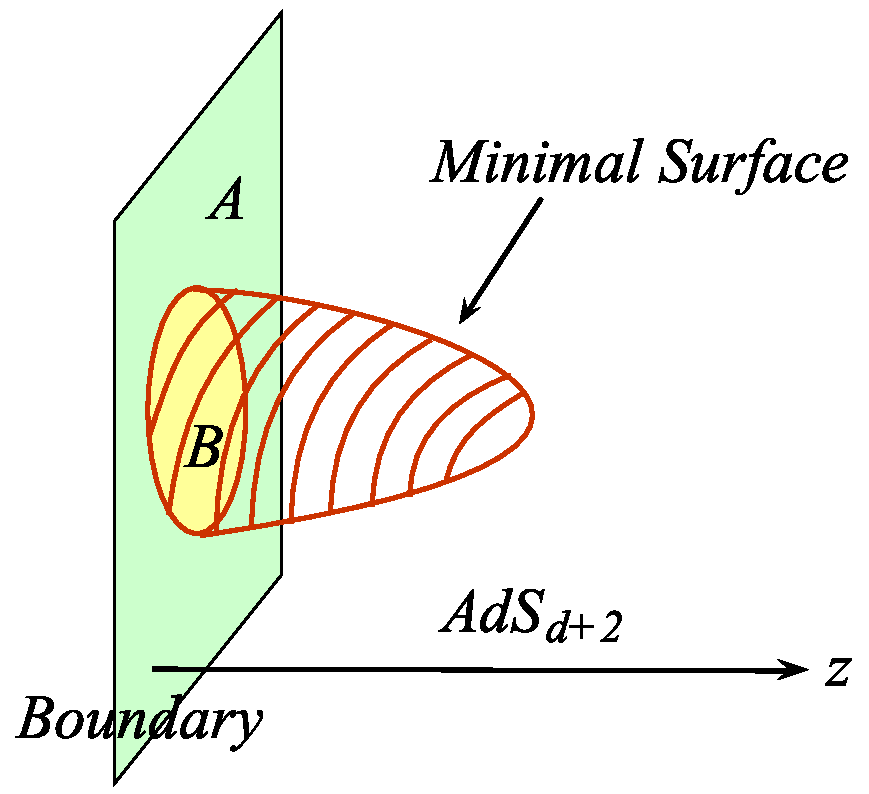
\includegraphics[width=0.4\textwidth]{images/operator-pushing/rt-formula.pdf}} \qquad
  \subcaptionbox{\label{fig:mera-ads-cft}}{%
    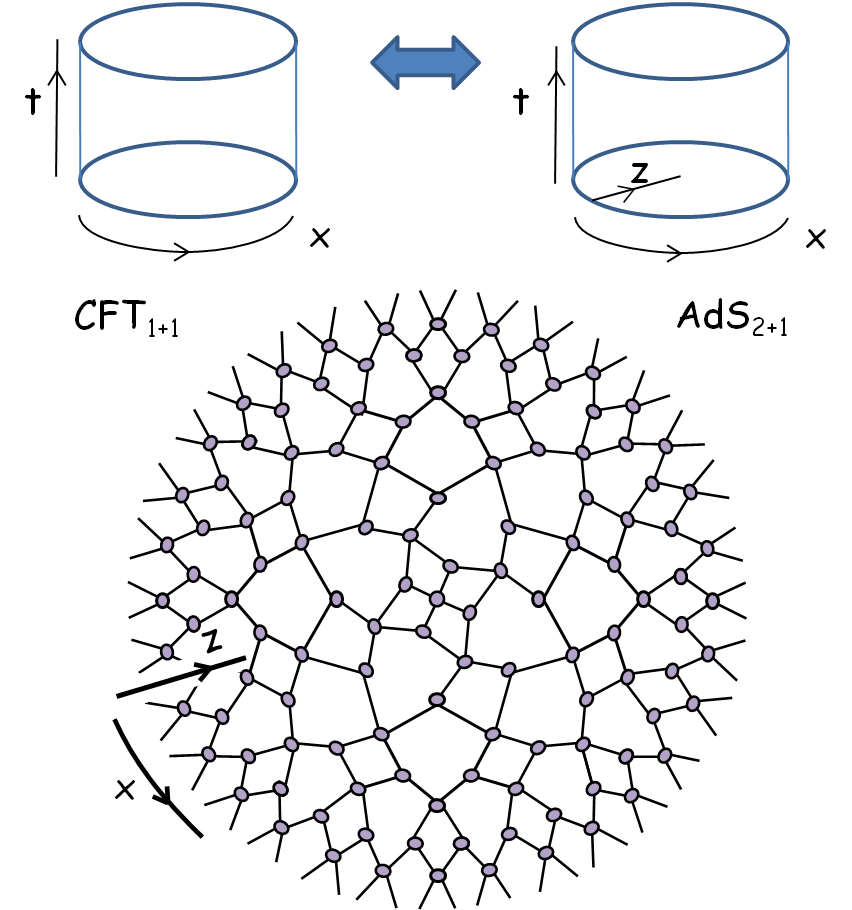
\includegraphics[width=0.35\textwidth]{images/operator-pushing/mera-ads-cft.pdf}}
  \caption[全息张量网络与 AdS/CFT 对应]{(a) Ryu--Takayanagi 公式 $S_A=\operatorname{Area}(\gamma_A)/4G$ 指出,$\text{CFT}_d$ 边界上的纠缠熵与 $\text{AdS}_{d+1}$ 时空中极小曲面 $\gamma_A$ 的面积成正比,其中 $G$ 为 $d+1$ 维中的 Newton 引力常数。图片来源:\parencite{nishioka2009holographic}。(b) MERA 张量网络可以被理解为 AdS/CFT 的一种离散实现。一维格点模型的基态波函数对应了 $\text{CFT}_{1+1}$ 的真空态,而由此“生长”出的二维 MERA 张量网络则给出了 $\text{AdS}_{2+1}$ 时间切片的一种离散表示。图片来源:\parencite{evenbly2011tensor}。}
\end{figure}

另一方面,受 Ryu--Takayanagi 公式\cite{ryu2006holographic,nishioka2009holographic}[图~\ref{fig:rt-formula}]的启发,也有人提出张量网络是构建 CFT 与 AdS 自由度之间线性映射的合适框架\cite{swingle2012entanglement}。而如图~\ref{fig:mera-ads-cft} 所示,这类张量网络的图形表示也和 AdS 空间的离散版本非常相似。它描述了 CFT 边界自由度的重整化(粗粒近似)过程,而这些自由度同时也位于张量网络的渐进边界。体中的算符作用在张量网络的辅助指标上,而 CFT 中的算符则作用在张量网络的渐进边界上。因此,张量网络提供了这些算符之间的线性映射\cite{pastawski2015holographic,hayden2016holographic}。

由于张量网络实际上是局域化的,它可以分解为一系列张量的乘积,而这些张量只与邻近的张量相缩并(邻近张量的数目则取决于体空间的维数),因而我们可以通过\emph{算符推移} (operator pushing) 的方法来找出相应的\emph{体—边映射} (bulk-boundary map)\cite{pastawski2015holographic,bhattacharyya2016exploring,bhattacharyya2018tensor}。

于是这就引出了一个自然的问题:对于一个弱耦合的体理论,其中的场几乎都是自由的,那么此时什么样的张量网络最能描述相应 AdS/CFT 中的体—边映射?文献 \parencite{bhattacharyya2018tensor} 对这个问题进行了一些讨论。如图~\ref{fig:operator-pushing} 所示,对于体中的算符 $\mathcal{O}$,它作用在体内部的自由度上;而当利用算符推移把 $\mathcal{O}$ 拉到边界时,这种作用应当等价于另一组算符 $\mathcal{O}'$ 在边界自由度上的作用。在利用边界算符对体算符进行重建时,我们有必要对入射、出射腿的方向做出选择。事实上,当张量网络对应了重整化(粗粒近似)操作时,这种选择是唯一的:作用在粗粒近似后的自由度上的算符,应当由作用在粗粒近似前的自由度上的算符来决定。此时可以证明,一个广义的自由场在利用算符推移穿过张量网络后,可以被分解为一系列\emph{简单算符} (simple operators) 之和\cite{bhattacharyya2018tensor}。

\begin{figure}[htb]
  \centering
  \subcaptionbox{}{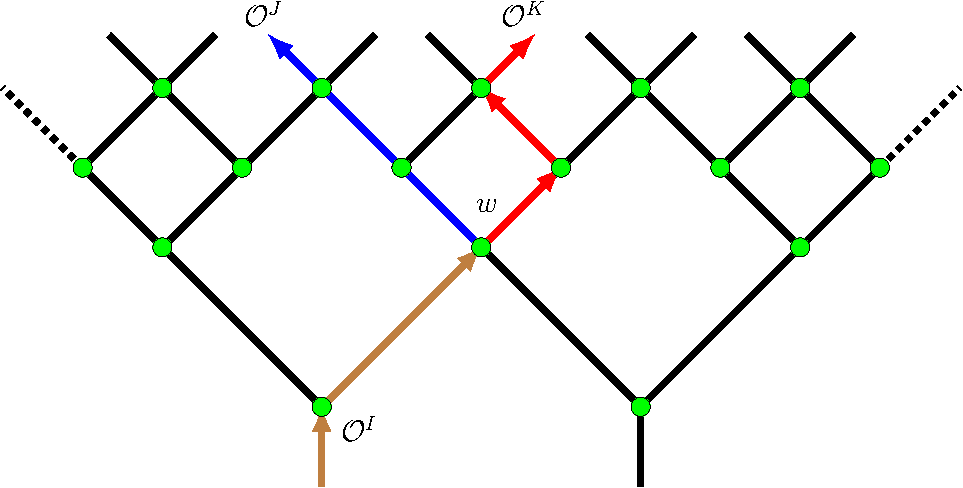
\includegraphics[width=0.45\textwidth]{images/operator-pushing/operator-pushing-1.pdf}} \quad
  \subcaptionbox{}{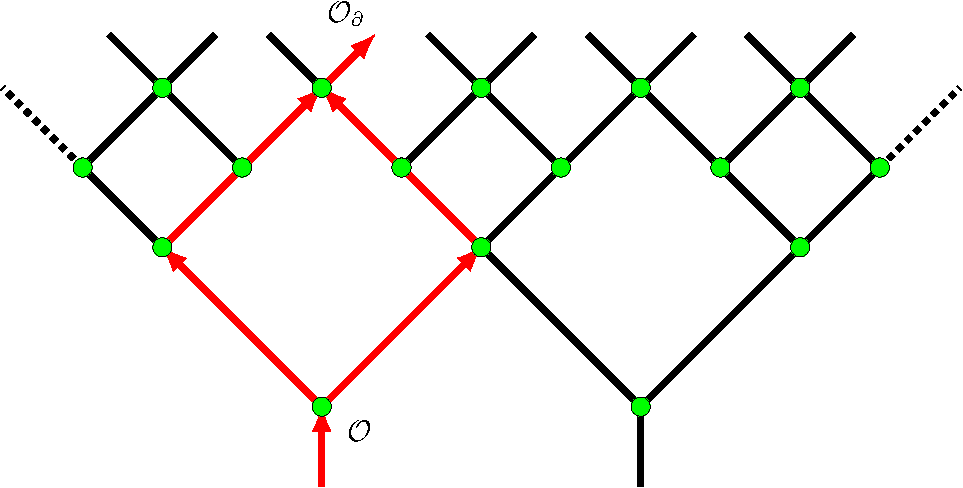
\includegraphics[width=0.45\textwidth]{images/operator-pushing/operator-pushing-2.pdf}}
  \caption[算符推移]{算符推移。(a) 体算符 $\mathcal{O}^I$ 由边界算符 $\mathcal{O}^J$ 和 $\mathcal{O}^K$ 重建。(b) 体算符 $\mathcal{O}$ 由简单形式的边界算符 $\mathcal{O}^\partial$ 重建,因而对应了广义自由场。图片来源:\parencite{bhattacharyya2018tensor}。}
  \label{fig:operator-pushing}
\end{figure}

考虑一个由重整化张量 $M^{i_1,\dots,i_K}_{j_1,\dots,j_H}\colon\mathbb{V}^K\to\mathbb{V}^H$ 构成的张量网络,其中 $K>H$,$i_l,j_l\in\mathbb{V}$,而 $\mathbb{V}$ 是一个 $d$ 维向量空间。那么算符推移对应于
\begin{equation}
  \mathcal{O} \bigl( \mathbb{V}^H \bigr) \cdot M = M \cdot \mathcal{O} \bigl( \mathbb{V}^K \bigr).
  \label{eq:operator-pushing}
\end{equation}
一个近似自由的体算符会作用在 $\mathbb{V}^H$ 其中一个指标上,即
\begin{equation}
    \mathcal{O} \bigl( \mathbb{V}^H \bigr)
  = \mathbb{I}_1 \otimes \cdots \otimes \mathbb{I}_{i-1} \otimes X_i \otimes \mathbb{I}_{i+1} \otimes \dots \otimes \mathbb{I}_{H}.
\end{equation}
当 $\mathcal{O}$ 满足式~\eqref{eq:operator-pushing} 时,则有
\begin{equation}
    \mathcal{O} \bigl( \mathbb{V}^K \bigr)
  = \sum_{i=1}^K \alpha_i \, \bigl(
      \mathbb{I}_1 \otimes \cdots \otimes \mathbb{I}_{i-1} \otimes X_i \otimes \mathbb{I}_{i+1} \otimes \dots \otimes \mathbb{I}_{K}
    \bigr),
  \label{eq:operator-pushing-coefficients}
\end{equation}
其中 $\{\alpha_i\}$ 为常数。此时,作用在体自由度 $l_B$ 上的体算符 $\mathcal{O}(l_B)$ 就可以用边界算符重建出来:
\begin{equation}
  \mathcal{O} \bigl( l_B \bigr) = \sum_b K^I \bigl( l_b, l_B \bigr) \, \mathcal{O}^I \bigl( l_b \bigr),
\end{equation}
其中 $\{\mathcal{O}^I\}$ 是作用在边界自由度 $l_b$ 上算符的一组完备基,而 $K^I(l_b, l_B)$ 是\emph{体—边核} (bulk-boundary kernel),它可用式~\eqref{eq:operator-pushing-coefficients} 中的系数 $\alpha_i$ 表示。可以发现,这一表达式与通过\emph{体—边传播子} (bulk-boundary propagator) 构造的 \emph{HKLL 核} (HKLL kernel)\cite{hamilton2006local,hamilton2006holographic}具有相同的形式。此外还可以证明,体算符关联函数的行为与广义自由场是类似的\cite{bhattacharyya2018tensor,hung2019padic}。由于 $M$ 是一个长方形的矩阵,所以这种重建不是唯一的。然而,只要式~\eqref{eq:operator-pushing-coefficients} 成立,那么广义自由场的解总是存在的。

\section{1+1 维中的算符推移}

我们首先讨论 1+1 维的情形,即由有限群 $G$ 所描述的 Dijkgraaf--Witten 理论。在 \ref{subsec:holographic-tensor-network-1+1d} 小节中,我们已经给出了重整化算符的构造。它对应了一个树状结构的张量网络,其中每个顶点都是三分支的。在无扭转的 Dijkgraaf--Witten 理论中,每个顶点对应了一个带有三个指标的张量 $M^{g_1g_2}_{g_3}$:
\begin{equation}
  \tikzinput{operator-pushing/tensor-1+1d},
\end{equation}
其中 $g_1$、$g_2$、$g_3$ 都是群 $G$ 中的元素。张量 $M$ 描述了 $G$ 中的群乘法(也相当于融合规则),即
\begin{equation}
  M^{ij}_k = \delta_{G(i,j), k}, \quad
  G(g_1, g_2) \coloneq g_1 \times g_2 = g_3.
\end{equation}

如图~\ref{fig:rg-1+1d} 所示,这一由重整化算符所构成的张量网络具有一维边界。当在体中插入一个算符 $B$ 时,它的作用应当等价于边界上插入的另外一些算符。找到能再现体算符作用的边界算符,也就是我们所说的算符推移或\emph{体算符重建} (bulk operator reconstruction) 问题。

由于张量网络是局域的,我们可以通过研究重整化张量网络中的一个张量来研究体算符重建。具体来说,对于一个张量单元而言,算符推移或重建相当于为给定的算符 $B$ 找到对应的算符 $A$,并使其满足
\begin{equation}
  \tikzinput{operator-pushing/constraint-1+1d}.
  \label{eq:1+1d-constraint}
\end{equation}
当算符 $B$ 是所谓广义自由场时,由 $A$ 给出的算符重建应当可以表示为“简单”形式(即 $\mathbb{I}\otimes\tilde{A}$ 或 $\tilde{A}\otimes\mathbb{I}$ 的线性组合)。为了确保 $B$ 的行为满足广义自由场的条件,我们还要求 $\tilde{A}$ 仍然属于算符集 $\{B\}$,也就是要求这一重建过程可以被不断重复至任意层的张量网络。式~\eqref{eq:1+1d-constraint} 可以表述为
\begin{equation}
  A_{(ij), (i'j')} M_{(i'j'), k} = M_{(ij), k'} B_{k', k}.
  \label{eq:1+1d-constraint-equation}
\end{equation}
为计算方便,我们把 $i$、$j$ 合并成了单个指标 $(ij)$,类似张量网络中的变形操作[式~\eqref{eq:tensor-reshape}]。接下来我们考虑对一般的算符 $B$ 求解式~\eqref{eq:1+1d-constraint-equation},并从中确定广义自由场的集合。还可以注意到,在张量网络中,如果算符 $A$ 能够表示为简单形式,则算符 $B$ 的集合将构成广义自由场的一组完备基。

在式~\eqref{eq:1+1d-constraint} 中张量的每条腿上,都有一个 $|G|$ 维的向量空间。作为 $\mathbb{Z}_2$ 情形中 Pauli 矩阵的推广,我们可以利用\emph{广义 Pauli 矩阵} (generalized Pauli matrices)\cite{patera1988pauli}作为基,来构建作用在每条腿上的算符。对于有限群 $G$ 且有 $|G|=n$,$G$ 中群元标记为 $0, 1, \dots, n-1$,则 $|G|$ 维的向量空间中的基可以表示为
\begin{equation}
  \ket{i} = \begin{pmatrix} 0 \\ \vdots \\ 1_{\text{$i$-th}} \\ \vdots \\ 0 \end{pmatrix}, \quad
  i \in \{ 0, 1, \dots, n-1 \}.
\end{equation}
在这组基下,广义 Pauli 矩阵可通过\emph{移位矩阵} (shift matrix) $X$ 和\emph{时钟矩阵} (clock matrix) $Z$ 生成:
\begin{equation}
  X = \begin{pmatrix}
    0      & 1      & 0      & \cdots & 0      \\
    0      & 0      & 1      & \cdots & 0      \\
    \vdots & \vdots & \vdots & \ddots & \vdots \\
    0      & 0      & 0      & \cdots & 1      \\
    1      & 0      & 0      & \cdots & 0
  \end{pmatrix}, \quad
  Z = \begin{pmatrix}
    1      & 0      & \cdots & 0            & 0      \\
    0      & \omega & \cdots & 0            & 0      \\
    \vdots & \vdots & \ddots & \vdots       & \vdots \\
    0      & 0      & \cdots & \omega^{n-2} & 0      \\
    0      & 0      & \cdots & 0            &\omega^{n-1}
  \end{pmatrix},
  \label{eq:generalized-pauli-matrices}
\end{equation}
这里 $\omega=\ee^{2\pi i/n}$ 是 $n$ 次单位根。于是广义 Pauli 矩阵为
\begin{equation}
  \sigma^\mu \coloneq \sigma^{ns+t} = X^t Z^s,
\end{equation}
其中 $s=\lfloor \mu/n\rfloor$、$t=\mu\bmod n$,而 $\mu\in\{0,1,\dots,n^2-1\}$。此时式~\eqref{eq:1+1d-constraint-equation} 可以写为
\begin{equation}
    A_{(ij), (i'j')} \delta_{G(i',j'), k}
  = \delta_{G(i,j), k'} B_{k', k}
  = \delta_{G(i,j), k'} \sigma^\mu_{k', k}
  = \sigma^\mu_{G(i,j), k}.
\end{equation}
因此,一旦给定了群乘法 $G(i,j)$,我们就可以根据标准的线性代数方法,对于每一个 $\sigma_\mu$ 求解上式中的 $A$。完整的解系应包含通解和特解两个部分,其中通解部分对应于齐次方程
\begin{equation}
  A_{(ij), (i'j')} \delta_{G(i',j'), k} = 0
\end{equation}
的解,即相当于 $(\sigma^\mu_{G(i,j),k})^{\mathrm{T}}=\sigma^\mu_{k,G(i,j)}$ 的\emph{零空间} (null space)。而注意到
\begin{equation}
  G(i,0) = i, \quad G(0,j) = j,
\end{equation}
我们可以给出一组特解:
\begin{equation}
  A^{(\mu)}_{(ij), (i'j')} = \begin{cases}
    \sigma^\mu_{G(i,j), j'}, & i' = 0; \\
    0, & i' \neq 0.
  \end{cases}
  \label{eq:1+1d-specific-solution}
\end{equation}

我们还想找到能使算符 $A$ 为简单形式的体算符 $B$ 的子集,此时要求 $A$ 在张量一条腿上的作用是平凡的,即
\begin{equation}
  A_{(ij), (i'j')} = \tilde{A}_{ii'} \delta_{jj'} \quad \text{or} \quad
  A_{(ij), (i'j')} = \delta_{ii'} \tilde{A}_{jj'}.
\end{equation}
于是有
\begin{equation}
  \tilde{A}_{ii'} \delta_{G(i',j), k} = \sigma^\mu_{G(i,j), k} \quad \text{or} \quad
  \tilde{A}_{jj'} \delta_{G(i,j'), k} = \sigma^\mu_{G(i,j), k}, \quad
  \forall j \in \{ 0, 1, \dots, n-1 \}.
  \label{eq:1+1d-simple-form-constraint-equation}
\end{equation}
$\tilde{A}$ 仍然可以很容易地求解得到。根据线性代数中的 Rouch\'e--Capelli 定理,上式有解的充分必要条件是对于 $(\sigma^\mu_{G(i,j),k})^{\mathrm{T}}$ 的每一列,增广矩阵的秩都满足
\begin{equation}
    \rank\bigl[ (\delta_{G(i',j), k})^{\mathrm{T}} \big| (\sigma^\mu_{G(i,j),k})^{\mathrm{T}}_s \bigr]
  = \rank\bigl[ (\delta_{G(i',j), k})^{\mathrm{T}} \bigr].
\end{equation}
又因为
\begin{equation}
    \rank\bigl[ (\delta_{G(i',j), k})^{\mathrm{T}} \bigr]
  = \rank\bigl( \delta_{G(i',j), k} \bigr) = n,
\end{equation}
如果式~\eqref{eq:1+1d-simple-form-constraint-equation} 有解,也只存在一组解。在实际计算中,我们可以取一组系数 $\{\alpha_\mu\}$,使得
\begin{equation}
  \tilde{A}_{ii'} \delta_{G(i',j), k} - \sum_\mu \alpha_\mu \sigma^\mu_{G(i,j), k} = 0,
  \label{eq:1+1d-simple-form-augmented-constraint-equation}
\end{equation}
这是一组同时以 $\tilde{A}_{ii'}$ 和 $\alpha_\mu$ 为变量的(齐次)方程。求解它即可得到符合要求的 $B=\sum_\mu\alpha_\mu\sigma^\mu$ 以及相应的算符 $A$。

\subsection{Abelian 的例子:\texorpdfstring{$\mathbb{Z}_n$}{ℤₙ} 群}

接下来我们考察几个具体的例子。对于 $\mathbb{Z}_n$ 群,其融合规则由模算术给出:
\begin{equation}
  G(i,j) = (i+j)\bmod n,
  \label{eq:Z_n-fusion-rules}
\end{equation}
因此 $\delta_{G(i,j),k}=\delta_{(i+j)\bmod n,k}$ 是一个秩为 $n$ 的 $n^2\times n$ 矩阵,其转置矩阵的零空间可由 $n^2-n$ 个向量 $\bm{v}$ 张成:
\begin{equation}
  v^{(p)}_q = \delta_{(-p-\lfloor p/n\rfloor-2)\bmod n, \, q} - \delta_{n^2-p-1, \, q},
\end{equation}
其中 $p\in\{0,1,\dots,n^2-n-1\}$,$q\in\{0,1,\dots,n^2-1\}$。于是通解 $A^*$ 可由 $v^{(p)}$ 的线性组合给出:
\begin{equation}
  A^* = \begin{pmatrix}
    \beta_{0,0} \bm{v}^{(0)} + \dots + \beta_{0,n^2-n-1} \bm{v}^{(n^2-n-1)} \\
    \vdots \\
    \beta_{n^2-1,0} \bm{v}^{(0)} + \dots + \beta_{n^2-1,n^2-n-1} \bm{v}^{(n^2-n-1)}
  \end{pmatrix},
\end{equation}
其中 $\beta_{i,j}$ 是任意常数。而根据式~\eqref{eq:1+1d-specific-solution},特解部分为
\begin{equation}
  A^{(\mu)}_{(ij), (0j')} = \sigma^\mu_{(i+j)\bmod n, j'}.
\end{equation}

对于算符 $A$ 为简单形式的情形,求解式~\eqref{eq:1+1d-simple-form-augmented-constraint-equation} 可知,对于 $\mu\geqslant n$,有 $\alpha_\mu=0$,这意味着 $\mu\in\{0,1,\dots,n-1\}$ 时式~\eqref{eq:1+1d-simple-form-constraint-equation} 有解。而此时
\begin{equation}
  \tilde{A}^{(\mu)}_{ii'} = \sigma_\mu.
\end{equation}
因而当且仅当 $B=\sigma_k$ 而 $k\in\{1,2,\dots,n-1\}$ 时($\sigma_0=\mathbb{I}$ 对应了同样是平凡算符的 $A=\mathbb{I}\otimes\mathbb{I}$,因此将其忽略),对应的
\begin{equation}
  A = \sigma_k   \otimes \mathbb{I} \quad \text{or} \quad
  A = \mathbb{I} \otimes \sigma_k
\end{equation}
为简单算符。由于 $\tilde{A}=\sigma_k$ 可以作为新一层的体算符 $B$,这样的算符推移操作可以不断进行下去。考虑一个 $L$ 层的张量网络(见图~\ref{fig:rg-1+1d}),对于上述的 $B=\sigma_k$,边界算符仍然具有简单形式,并且可以写为:
\begin{equation}
  A_L = \mathbb{I}^{\otimes L-l} \otimes \sigma_k \otimes \mathbb{I}^{\otimes l-1}, \quad l = 0,1,\dots,L.
\end{equation}

下面我们以 $\mathbb{Z}_2$ 群(即 $n=2$)为例给出一个具体的解。$\delta_{k,(i+j)\bmod 2}$ 的零空间可以由向量组
\begin{equation}
  \{ v^{(p)} \} = \Biggl\{ \,
    \begin{pmatrix} 1 \\ 0 \\ 0 \\ -1 \end{pmatrix}, \,
    \begin{pmatrix} 0 \\ 1 \\ -1 \\ 0 \end{pmatrix} \,
  \Biggr\}
\end{equation}
张成,这等价于通解
\begin{equation}
  A^* = \begin{pmatrix}
    \beta_{0,0} & \beta_{0,1} & -\beta_{0,1} & -\beta_{0,0} \\
    \beta_{1,0} & \beta_{1,1} & -\beta_{1,1} & -\beta_{1,0} \\
    \beta_{2,0} & \beta_{2,1} & -\beta_{2,1} & -\beta_{2,0} \\
    \beta_{3,0} & \beta_{3,1} & -\beta_{3,1} & -\beta_{3,0}
  \end{pmatrix},
\end{equation}
其中 $\beta_{i,j}$ 是任意常数。因而完整的解可以表示为
\begin{align}
  B = \sigma_0 = \mathbb{I}   &\implies A = A^* + \begin{pmatrix} 1 &  0 & 0 & 0 \\ 0 &  1 & 0 & 0 \\ 0 &  1 & 0 & 0 \\ 1 &  0 & 0 & 0 \end{pmatrix}, \notag \displaybreak[0] \\
  B = \sigma_1 = \sigma_x     &\implies A = A^* + \begin{pmatrix} 0 &  1 & 0 & 0 \\ 1 &  0 & 0 & 0 \\ 1 &  0 & 0 & 0 \\ 0 &  1 & 0 & 0 \end{pmatrix}, \notag \displaybreak[0] \\
  B = \sigma_2 = \sigma_z     &\implies A = A^* + \begin{pmatrix} 1 &  0 & 0 & 0 \\ 0 & -1 & 0 & 0 \\ 0 & -1 & 0 & 0 \\ 1 &  0 & 0 & 0 \end{pmatrix}, \notag \displaybreak[0] \\
  B = \sigma_3 = -\ii\sigma_y &\implies A = A^* + \begin{pmatrix} 0 & -1 & 0 & 0 \\ 1 &  0 & 0 & 0 \\ 1 &  0 & 0 & 0 \\ 0 & -1 & 0 & 0 \end{pmatrix}.
  \label{eq:Z_2-solution}
\end{align}
可以看到当且仅当体算符 $B=\sigma_x$ 时,边界算符 $A$ 可以取到简单形式
\begin{equation}
  A = \mathbb{I} \otimes \sigma_x = \begin{pmatrix}
    0 & 1 & 0 & 0 \\
    1 & 0 & 0 & 0 \\
    0 & 0 & 0 & 1 \\
    0 & 0 & 1 & 0
  \end{pmatrix}
  \quad \text{or} \quad
  A = \sigma_x \otimes \mathbb{I} = \begin{pmatrix}
    0 & 0 & 1 & 0 \\
    0 & 0 & 0 & 1 \\
    1 & 0 & 0 & 0 \\
    0 & 1 & 0 & 0
  \end{pmatrix}.
\end{equation}

\subsection{非 Abelian 的例子:\texorpdfstring{$S_3$}{𝑆₃} 群}

$S_3$ 群的乘法表为:
\begin{center}
  \begin{tabular}{c|cccccc}
    & $g_0$ & $g_1$ & $g_2$ & $g_3$ & $g_4$ & $g_5$ \\
    \hline
    $g_0$ & 0 & 1 & 2 & 3 & 4 & 5 \\
    $g_1$ & 1 & 0 & 3 & 2 & 5 & 4 \\
    $g_2$ & 2 & 4 & 0 & 5 & 1 & 3 \\
    $g_3$ & 3 & 5 & 1 & 4 & 0 & 2 \\
    $g_4$ & 4 & 2 & 5 & 0 & 3 & 1 \\
    $g_5$ & 5 & 3 & 4 & 1 & 2 & 0 \\
  \end{tabular}
\end{center}
我们取
\begin{equation}
  G(i,j) = g_i g_j,
\end{equation}
则可知 $G(1,2)=g_1 g_2=g_3\eqcolon3$,$G(2,1)=g_2 g_1=g_4\eqcolon4$,显然关于 $i$、$j$ 不对称。

这里我们主要关注简单形式的解。此时式~\eqref{eq:1+1d-simple-form-augmented-constraint-equation} 的系数矩阵大小为 $216\times72$,而其秩为 66,因而存在 6 组解,分别为
\begin{align}
  B^{(0)} &= \sigma_0, \notag \\
  B^{(1)} &= \sigma_1 + \sigma_2 + \sigma_3 + \sigma_4 + \sigma_5, \notag \\
  B^{(2)} &= \sigma_2 + \sigma_3 + \sigma_4 + \sigma_{19} - \sigma_{23}, \notag \\
  B^{(3)} &= \frac13 \, \bigl[
        (\sigma_2 + \sigma_3 + \sigma_4 + \sigma_{16} + \sigma_{28})
      - \omega \, (\sigma_{15} + \sigma_{26})
      + \omega^2  (\sigma_{14} + \sigma_{27})
    \bigr], \notag \\
  B^{(4)} &= \frac{1}{2\sqrt{3}} \Bigl(
        \ii \sigma_3
      + \frac{2}{\sqrt{3}} \ee^{\frac{\ii\pi}{3}} \sigma_8
      + \ee^{-\frac{5 \ii\pi}{6}} \sigma_9
      - \frac{1}{\sqrt{3}} \sigma_{10}
      + \ee^{-\frac{\ii\pi}{6}} \sigma_{11}
      - \ii \sigma_{13}
      + \ii \sigma_{16} \notag \\
    &\quad {}
      + \frac{1}{\sqrt{3}} \sigma_{20}
      - \frac{1}{\sqrt{3}} \sigma_{22}
      + \ee^{-\frac{\ii\pi}{6}} \sigma_{26}
      + \ee^{\frac{5 \ii\pi}{6}} \sigma_{29}
      - \ii \sigma_{31}
      + \frac{1}{\sqrt{3}} \ee^{\frac{2\ii\pi}{3}} \sigma_{32}
      + \ee^{\frac{5 \ii\pi}{6}} \sigma_{33}
      + \frac{2}{\sqrt{3}} \sigma_{34}
    \Bigr), \notag \\
  B^{(5)} &= \frac12 \Bigl(
        2 \ee^{\frac{\ii\pi}{3}} \sigma_2
      + \ee^{\frac{\ii\pi}{3}} \sigma_3
      + 2 \ee^{\frac{\ii\pi}{3}} \sigma_4
      + 2 \ee^{\frac{\ii\pi}{3}} \sigma_7
      - 3 \sigma_9 \notag \\
    &\quad {}
      + \sqrt{3} \ee^{-\frac{\ii\pi}{6}} \sigma_{10}
      + \ee^{-\frac{\ii}{3}} \sigma_{11}
      + \ee^{-\frac{2\ii\pi}{3}} \sigma_{13}
      + 2 \ee^{-\frac{\ii}{3}} \sigma_{15}
      + 3 \ee^{\frac{\ii\pi}{3}} \sigma_{16}
      - 2 \sigma_{17} \notag \\
    &\quad {}
      + \sqrt{3} \ee^{-\frac{\ii\pi}{6}} \sigma_{20}
      + \sqrt{3} \ee^{\frac{5\ii\pi}{6}} \sigma_{22}
      + 2 \ee^{\frac{\ii\pi}{3}} \sigma_{25}
      + 3 \ee^{-\frac{\ii}{3}} \sigma_{26}
      - 2 \sigma_{27} \notag \\
    &\quad {}
      + \ee^{\frac{2\ii\pi}{3}} \sigma_{29}
      + \ee^{-\frac{2\ii\pi}{3}} \sigma_{31}
      - i \sqrt{3} \sigma_{32}
      + 3 \ee^{\frac{2\ii\pi}{3}} \sigma_{33}
      + 2 \sigma_{35}
    \Bigr).
\end{align}
对应的算符 $\tilde{A}$ 则为:
\begin{align}
  \tilde{A}^{(0)} &= \begin{pmatrix}
    1 & 0 & 0 & 0 & 0 & 0 \\
    0 & 1 & 0 & 0 & 0 & 0 \\
    0 & 0 & 1 & 0 & 0 & 0 \\
    0 & 0 & 0 & 1 & 0 & 0 \\
    0 & 0 & 0 & 0 & 1 & 0 \\
    0 & 0 & 0 & 0 & 0 & 1
  \end{pmatrix}
  = \sigma_0 = B^{(0)}, \notag \displaybreak[0] \\
  \tilde{A}^{(1)} &= \begin{pmatrix}
    0 & 1 & 1 & 1 & 1 & 1 \\
    1 & 0 & 1 & 1 & 1 & 1 \\
    1 & 1 & 0 & 1 & 1 & 1 \\
    1 & 1 & 1 & 0 & 1 & 1 \\
    1 & 1 & 1 & 1 & 0 & 1 \\
    1 & 1 & 1 & 1 & 1 & 0
  \end{pmatrix}
  = \sigma_1 + \sigma_2 + \sigma_3 + \sigma_4 + \sigma_5 = B^{(1)}, \notag \displaybreak[0] \\
  \tilde{A}^{(2)} &= \begin{pmatrix}
    0 & -1 & 1 & 1 & 1 & 1 \\
    -1 & 0 & 1 & 1 & 1 & 1 \\
    1 & 1 & 0 & -1 & 1 & 1 \\
    1 & 1 & -1 & 0 & 1 & 1 \\
    1 & 1 & 1 & 1 & 0 & -1 \\
    1 & 1 & 1 & 1 & -1 & 0
  \end{pmatrix}
  = \sigma_2 + \sigma_3 + \sigma_4 + \sigma_{19} - \sigma_{23} = B^{(2)}, \notag \displaybreak[0] \\
  \tilde{A}^{(3)} &= \begin{pmatrix}
    0 & 0 & 1 & 0 & 0 & 0 \\
    0 & 0 & 0 & 0 & 1 & 0 \\
    1 & 0 & 0 & 0 & 0 & 0 \\
    0 & 0 & 0 & 0 & 0 & 1 \\
    0 & 1 & 0 & 0 & 0 & 0 \\
    0 & 0 & 0 & 1 & 0 & 0
  \end{pmatrix}
  = B^{(3)}, \notag \displaybreak[0] \\
  \tilde{A}^{(4)} &= \begin{pmatrix}
    0 & 0 & \frac{\ii}{2} & \ee^{\frac{i \pi }{6}} & \ee^{\frac{5\ii\pi}{6}} & -\ii \\[1ex]
    0 & 0 & \ee^{\frac{5\ii\pi}{6}} & -\ii & \frac{\ii}{2} & \ee^{\frac{i \pi }{6}} \\[1ex]
    \frac{\ii}{2} & \ee^{\frac{i \pi }{6}} & 0 & 0 & -\ii & \ee^{\frac{5\ii\pi}{6}} \\[1ex]
    \ee^{\frac{5\ii\pi}{6}} & -\ii & 0 & 0 & \ee^{\frac{i \pi }{6}} & \frac{\ii}{2} \\[1ex]
    \ee^{\frac{i \pi }{6}} & \frac{\ii}{2} & -\ii & \ee^{\frac{5\ii\pi}{6}} & 0 & 0 \\[1ex]
    -\ii & \ee^{\frac{5\ii\pi}{6}} & \ee^{\frac{i \pi }{6}} & \frac{\ii}{2} & 0 & 0
  \end{pmatrix}
  = B^{(4)}, \notag \displaybreak[0] \\
  \tilde{A}^{(5)} &= \begin{pmatrix}
    0 & 0 & \frac{5}{2} \ee^{\frac{\ii\pi}{3}} & 2-\ii\sqrt{3} & \frac{\ii(\sqrt{3}+5\ii)}{2} & \ee^{\frac{\ii\pi}{3}} \\[1ex]
    0 & 0 & \frac{\ii(\sqrt{3}+5\ii)}{2} & \ee^{\frac{\ii\pi}{3}} & \frac{5}{2} \ee^{\frac{\ii\pi}{3}} & 2-\ii\sqrt{3} \\[1ex]
    \frac{5}{2} \ee^{\frac{\ii\pi}{3}} & 2-\ii\sqrt{3} & 0 & 0 & \ee^{\frac{\ii\pi}{3}} & \frac{\ii(\sqrt{3}+5\ii)}{2} \\[1ex]
    \frac{\ii(\sqrt{3}+5\ii)}{2} & \ee^{\frac{\ii\pi}{3}} & 0 & 0 & 2-\ii\sqrt{3} & \frac{5}{2} \ee^{\frac{\ii\pi}{3}} \\[1ex]
    2-\ii\sqrt{3} & \frac{5}{2} \ee^{\frac{\ii\pi}{3}} & \ee^{\frac{\ii\pi}{3}} & \frac{\ii(\sqrt{3}+5\ii)}{2} & 0 & 0 \\[1ex]
    \ee^{\frac{\ii\pi}{3}} & \frac{\ii(\sqrt{3}+5\ii)}{2} & 2-\ii\sqrt{3} & \frac{5}{2} \ee^{\frac{\ii\pi}{3}} & 0 & 0
  \end{pmatrix}
  = B^{(5)}.
\end{align}
可以发现这些 $\tilde{A}^{(i)}$ 和对应的 $B^{(i)}$ 恰好相等,因此算符推移的操作可以不断进行。并且与 $\mathbb{Z}_n$ 的情况相同,简单形式解的个数(即广义自由场的个数)也和群的阶数一致。

\section{2+1 维中的算符推移}

上一节中的讨论可以推广到更高的维度。从弦网模型出发,2+1 维的全息张量网络可利用奇异关联子来构建(见 \ref{subsec:holographic-tensor-network-2+1d} 小节),而其中的张量单元则可以表示为一系列的四面体[图~\ref{fig:tetrahedra-1}]。

\begin{figure}[htb]
  \centering
  \subcaptionbox{\label{fig:tetrahedra-1}}{\tikzinput{operator-pushing/tetrahedra-1}} \qquad
  \subcaptionbox{\label{fig:tetrahedra-2}}{\tikzinput{operator-pushing/tetrahedra-2}}
  \caption[2+1 维全息张量网络中的四面体张量单元]{2+1 维全息张量网络中的四面体张量单元。(a) 两个并列的四面体,上表面对应边界层,下表面则对应体层。(b) 单个四面体中,$a$、$b$、$c$、$i$、$j$、$k$ 为边指标,而 $I=\Phi(b,c,a)$ 为面指标。}
\end{figure}

作为一个粗粒近似(重整化)的映射,这个四面体单元将边 $i$、$j$、$m$、$n$ 投影到 $a$,并保持 $b$、$c$、$d$、$e$ 不变。于是在 2+1 维中,算符重建的问题就可以表述为:当在边 $a$ 上插入一个体算符 $B$ 时,相应的边界算符 $A$(作用在边 $i$、$j$、$m$、$n$ 上)是什么?$A$ 又能否表示成简单形式(对应 $B$ 为广义自由场)?

每个四面体有 6 条边,它们以张量融合范畴中的简单对象来标记,而四面体则被赋予一个相应的 $F$ 符号。如果其上的每个三角形都满足融合规则,则这个 $F$ 符号是非零的。考虑到融合规则的约束,为了方便计算,在处理体算符时我们可以将面指标而非边指标作为基本的自由度。于是在图~\ref{fig:tetrahedra-1} 中,我们可以认为体算符 $B$ 作用在三角形 $\overline{abc}$ 或 $\overline{ade}$ 上。

由于图~\ref{fig:tetrahedra-1} 中的两个四面体是对称的,我们可以只考虑其中一个,例如 $\overline{abcinm}$,另一个则可以通过翻转所有边来得到。如图~\ref{fig:tetrahedra-2} 所示,接下来我们选取这样的约定:小写字母 $i,j\in\{0,1,\dots,n-1\}$ 表示边指标,其中 $n$ 为融合范畴中简单对象的数目;大写字母 $I, J\in \{0,1,\dots,N-1\}$ 表示面指标(对应三角形或融合树),而 $N$ 则为融合规则所允许的三角形数目。面指标也可以用边指标来表示:
\begin{equation}
  I = \Phi(b,c,a),
\end{equation}
其中的 $\Phi$ 根据融合规则决定。

类似于 1+1 维中的式~\eqref{eq:1+1d-constraint-equation},2+1 维中的约束方程为:
\begin{equation}
    A_{(ijk), (i'j'k')} M_{(i'j'k'), I}
  = M_{(ijk), I'} B_{I', I}
  = M_{(ijk), I'} \sigma^\mu_{I', I},
\end{equation}
其中 $\mu\in\{0,1,\dots,N^2-1\}$。矩阵 $\bm{M}$ 则由式~\eqref{eq:tetrahedra-symbol} 给出:
\begin{equation}
  M_{(ijk), I} = M_{(ijk), \Phi(b,c,a)} = \sqrt{d_j d_k d_b d_c} \, \bigl[ F^{jkb}_c \bigr]_{ia},
\end{equation}
其中 $[F^{jkb}_c]_{ia}$ 为 $F$ 符号,而 $q_i$ 则为融合范畴中简单对象 $i$ 对应的量子维数。

同理,为了检查 $A$ 是否能表示为简单算符的形式,我们考虑如下形式的 $A$:
\begin{equation}
  A_{(ijk), (i'j'k')} = \tilde{A}_{ii'} \delta_{jj'} \delta_{kk'},
\end{equation}
并使其满足
\begin{equation}
  \tilde{A}_{ii'} M_{(i'jk), I} = M_{(ijk), I'} \sigma^\mu_{I', I}, \quad
  \forall j, k \in \{ 0, 1, \dots, n-1 \}.
\end{equation}
该式有解的条件为
\begin{equation}
  \rank\bigl[(M_{(i'jk), I})^{\mathrm{T}} | (M_{(ijk), I'} \sigma^\mu_{I', I})^{\mathrm{T}}_s \bigr] = \rank\bigl( M_{(i'jk), I} \bigr).
\end{equation}
我们同样也可以将其改写为
\begin{equation}
  \tilde{A}_{ii'} M_{(i'jk), I} - \sum_\mu \alpha_\mu M_{(ijk), I'} \sigma^\mu_{I', I} = 0
  \label{eq:2+1d-simple-form-augmented-constraint-equation}
\end{equation}
的形式,从而具体解出算符 $B$。而令指标 $i$、$j$ 或 $i$、$k$ 相同则可以获得其他简单算符的解。

\subsection{例子:\texorpdfstring{$\mathbb{Z}_n$}{ℤₙ} 模型}

我们仍然先由 $\mathbb{Z}_n$ 群所给出的融合范畴开始。四面体边上的自由度同样选取为 $\mathbb{Z}_n$ 中的群元,而面指标由式~\eqref{eq:Z_n-fusion-rules} 决定。以 $\mathbb{Z}_2$ 为例,其允许的融合规则(相当于三角形)为
\begin{equation}
  \Fusion000 \to 0, \quad
  \Fusion011 \to 1, \quad
  \Fusion101 \to 2, \quad
  \Fusion110 \to 3.
  \label{eq:Z_2-fusion-trees}
\end{equation}
此时面指标 $I$ 可以取值 0、1、2 或 3。一般地,我们有
\begin{equation}
  I = nb + c = n [(i+j)\bmod n] + [(i+k)\bmod n],
\end{equation}
其中 $i$、$j$ 为三角形的两条边[例如式~\eqref{eq:Z_2-fusion-trees} 中上面的两个指标]。可以发现 $N=n^2$,即面指标 $I$ 的取值范围为 $\{0,1,\dots,n^2-1\}$。

考虑平凡的 $\mathbb{Z}_n$ Dijkgraaf--Witten 模型,其中所有合法的(即被融合规则所允许)$F$ 符号都等于 1。这时可有
\begin{equation}
  M_{(ijk), I} = \delta_{n[(i+j)\bmod n]+[(i+k)\bmod n], I}.
\end{equation}
于是约束方程为
\begin{equation}
    A_{(ijk), (i'j'k')} \delta_{n[(i'+j')\bmod n]+[(i'+k')\bmod n], I}
  = \sigma^\mu_{n[(i+j)\bmod n]+[(i+k)\bmod n], I}.
\end{equation}
计算可知 $\bm{M}$ 的秩为 $n^2$,因而其转置矩阵的零空间可由 $n^3-n^2$ 个向量 $\bm{v}$ 张成:
\begin{equation}
    v^{(p)}_q
  = \delta_{n [(- \lfloor p/n\rfloor - \lfloor p/n^2 \rfloor - 2) \bmod n] + [(- \lfloor p/n^2 \rfloor - 2) \bmod n], q}
  - \delta_{n^3-p-1, q},
\end{equation}
其中 $p\in\{0,1,\dots,n^3-n^2-1\}$,$q\in\{0,1,\dots,n^3-1\}$。特解部分则为
\begin{equation}
  A^{(\mu)}_{(ijk), (0j'k')} = \sigma^\mu_{n[(i+j)\bmod n]+[(i+k)\bmod n], nj'+k'}.
\end{equation}

对于简单算符的求解,我们考察式~\eqref{eq:2+1d-simple-form-augmented-constraint-equation},其系数矩阵大小为 $n^5\times(n^4+n^2)$,而秩为 $n^4+n^2-n$,因此其零空间可由 $n$ 个向量张成。由于对一般的 $n$ 求解式~\eqref{eq:2+1d-simple-form-augmented-constraint-equation} 是困难的,下面我们仅给出 $n=2$ 和 3 的情况。$n=2$ 时,解为
\begin{align}
  B^{(0)} &= \sigma_0
    \implies \tilde{A}^{(0)} = \begin{pmatrix} 1 & 0 \\ 0 & 1 \end{pmatrix} = \sigma_0, \notag \\
  B^{(1)} &= \frac12 \bigl( \sigma_1 + \sigma_3 + \sigma_9 - \sigma_{11} \bigr)
    \implies \tilde{A}^{(1)} = \begin{pmatrix} 0 & 1 \\ 1 & 0 \end{pmatrix} = \sigma_1.
\end{align}
而 $n=3$ 时,解为
\begin{align}
  B^{(0)} &= \sigma_0
    \implies \tilde{A}^{(0)} = \begin{pmatrix} 1 & 0 & 0 \\ 0 & 1 & 0 \\ 0 & 0 & 1 \end{pmatrix} = \sigma_0, \notag \\
  B^{(1)} &= \frac13 \bigl( \sigma_1 + 2\sigma_4 + \sigma_{28} - \sigma_{31} + \sigma_{55} - \sigma_{58} \bigr)
    \implies \tilde{A}^{(1)} = \begin{pmatrix} 0 & 1 & 0 \\ 0 & 0 & 1 \\ 1 & 0 & 0 \end{pmatrix} = \sigma_1, \notag \\
  B^{(2)} &= \frac13 \Bigl[
      2\sigma_5 + \sigma_8 + \ee^{-\frac{\ii\pi}{3}} \bigl( \sigma_{32} - \sigma_{35} \bigr)
    - \ee^{-\frac{2\ii\pi}{3}} \bigl( \sigma_{59} - \sigma_{62} \bigr)
  \Bigr] \notag \\
    &\quad \implies \tilde{A}^{(1)} = \begin{pmatrix} 0 & 0 & 1 \\ 1 & 0 & 0 \\ 0 & 1 & 0 \end{pmatrix} = \sigma_2.
\end{align}
% \begin{equation}
%   B = \frac1n \left[ n \sigma_{n+1} + \sum_{k=0}^{n-1} \bigl( \sigma_{kn^3+1} - \sigma_{kn^3+n+1} \bigr) \right] \implies
%   A = \sigma_1 \otimes \mathbb{I} \otimes \mathbb{I}.
% \end{equation}

\subsection{例子:Fibonacci 模型}

最后我们考察一个 2+1 维拓扑序中的例子,即 Fibonacci 模型。它包含了 $\1$ 和 $\tau$ 两种简单对象,并满足融合规则
\begin{equation}
  \1 \times \1 = \1, \quad
  \1 \times \tau = \tau \times \1 = \tau, \quad
  \tau \times \tau = \1 + \tau,
\end{equation}
因此有 5 种允许的三角形(面指标):
\begin{equation}
  \Fusion000 \to 0, \quad
  \Fusion011 \to 1, \quad
  \Fusion101 \to 2, \quad
  \Fusion110 \to 3, \quad
  \Fusion111 \to 4.
\end{equation}
非零的 $F$ 符号为
\begin{equation}
  [F^{\tau\tau\tau}_\tau]_{ij} = \begin{pmatrix}
    \varphi^{-1}   &  \varphi^{-1/2} \\
    \varphi^{-1/2} & -\varphi^{-1}
  \end{pmatrix}, \quad
  i,j \in \{\1, \tau\},
\end{equation}
其中 $\varphi=(1+\sqrt5)/2$ 是黄金比。此时矩阵 $\bm{M}$ 可以显式地写为:
\begin{equation}
  M_{(ijk), I} = \begin{pmatrix}
    1 & 0 & 0 & 0 & 0 \\
    0 & 0 & \phi & 0 & 0 \\
    0 & 0 & 0 & \phi & 0 \\
    0 & \phi & 0 & 0 & \phi^{3/2} \\
    0 & \phi & 0 & 0 & 0 \\
    0 & 0 & 0 & \phi & \phi^{3/2} \\
    0 & 0 & \phi & 0 & \phi^{3/2} \\
    \phi & \phi^{3/2} & \phi^{3/2} & \phi^{3/2} & -\phi
  \end{pmatrix}.
\end{equation}
可以知道 $\rank(\bm{M})=5$,而 $\bm{M}^{\mathrm{T}}$ 的零空间则由向量组
\begin{equation}
  \{ v^{(p)} \} = \Biggl\{ \,
    \begin{pmatrix} \phi^{1/2} \\ 1 \\ 1 \\ -\phi^{-1} \\ \phi \\ 0 \\ 0 \\ -\phi^{1/2} \end{pmatrix}, \,
    \begin{pmatrix} 0 \\ 1 \\ 0 \\ 1 \\ -1 \\  0 \\ -1 \\ 0 \end{pmatrix}, \,
    \begin{pmatrix} 0 \\ 0 \\ 1 \\ 1 \\ -1 \\ -1 \\  0 \\ 0 \end{pmatrix} \,
  \Biggr\}
\end{equation}
张成。特解部分以及完整的解系可以通过数值方法给出,具体结果此处从略。

对于简单形式的解,我们仍然利用式~\eqref{eq:2+1d-simple-form-augmented-constraint-equation},此时系数矩阵大小为 $32\times20$,而秩为 19,这也就意味着仅存在一组解,但它同时是平凡的(即 $A=B=\mathbb{I}$)。因此在 Fibonacci 模型中并不存在广义自由场。

\section{本章小结}

本章探讨了在多种基于拓扑序的全息张量网络中演生出的广义自由场。对于 1+1 维和 2+1 维中几类具体的模型,我们求解得到了算符推移或算符重建的一般形式,并给出了边界算符为简单形式时所满足的条件。对于 1+1 维中的 $Z_n$ 群和 $S_3$ 群(它们都是具有平凡上同调类的 Dijkgraaf--Witten 模型),我们还证明了广义自由场(即对应简单形式边界算符的体算符)的数目,和群的阶数 $|G|$ 一致(将平凡算符 $\mathbb{I}$ 也考虑在内)。
